\section{Motivation}\label{sec:motivation}

\subsection{Background}

The standard approach to FDE, using the AES \emph{block cipher}, introduces
significant overhead during filesystem operation. It is well known that
authenticated encryption using \emph{stream ciphers} like
ChaCha20~\cite{ChaCha20} is faster than using AES~\cite{StrongBox, AnotherPaper,
AnotherPaper}. However, when used naively in drive encryption, stream ciphers
are vulnerable to ``overwrite attacks'' like two-time pad and
rollback~\cite{StrongBox}. To enable FDE using stream ciphers, several
approaches have been explored:

\begin{itemize}
   \item Use a non-deterministic CTR mode with specially designed cipher and
   filesystem (Freestyle~\cite{Freestyle}).
   \item Use a length-preserving ``tweakable super-pseudorandom permutation''
   with nonce-accepting stream cipher (Adiantum~\cite{Adiantum}).
   \item Use any stream cipher in a CTR-like mode with metadata management to
   prevent overwrites (StrongBox~\cite{StrongBox}).
\end{itemize}

In this paper, we focus on the lattermost approach. StrongBox~\cite{StrongBox}
is a stream cipher-based FDE and metadata layer that exploits Log-structured
File Systems' (LFS) overwrite-averse behavior to achieve high-performance
encryption using stream ciphers in a CTR-like mode to generate one-time
pads~\cite{OTP}. Threats like two-time pad and rollback---caused by
overwrites---are mitigated with \emph{re-keying}, where groups of contiguous
sectors referred to as \emph{nuggets} are re-encrypted with a new key when an
overwrite is detected. Overwrite-averse LFS behavior ensures costly re-keying
operations are triggered as rarely as possible during I/O~\cite{StrongBox}.

\begin{figure}[ht]
   \centering
   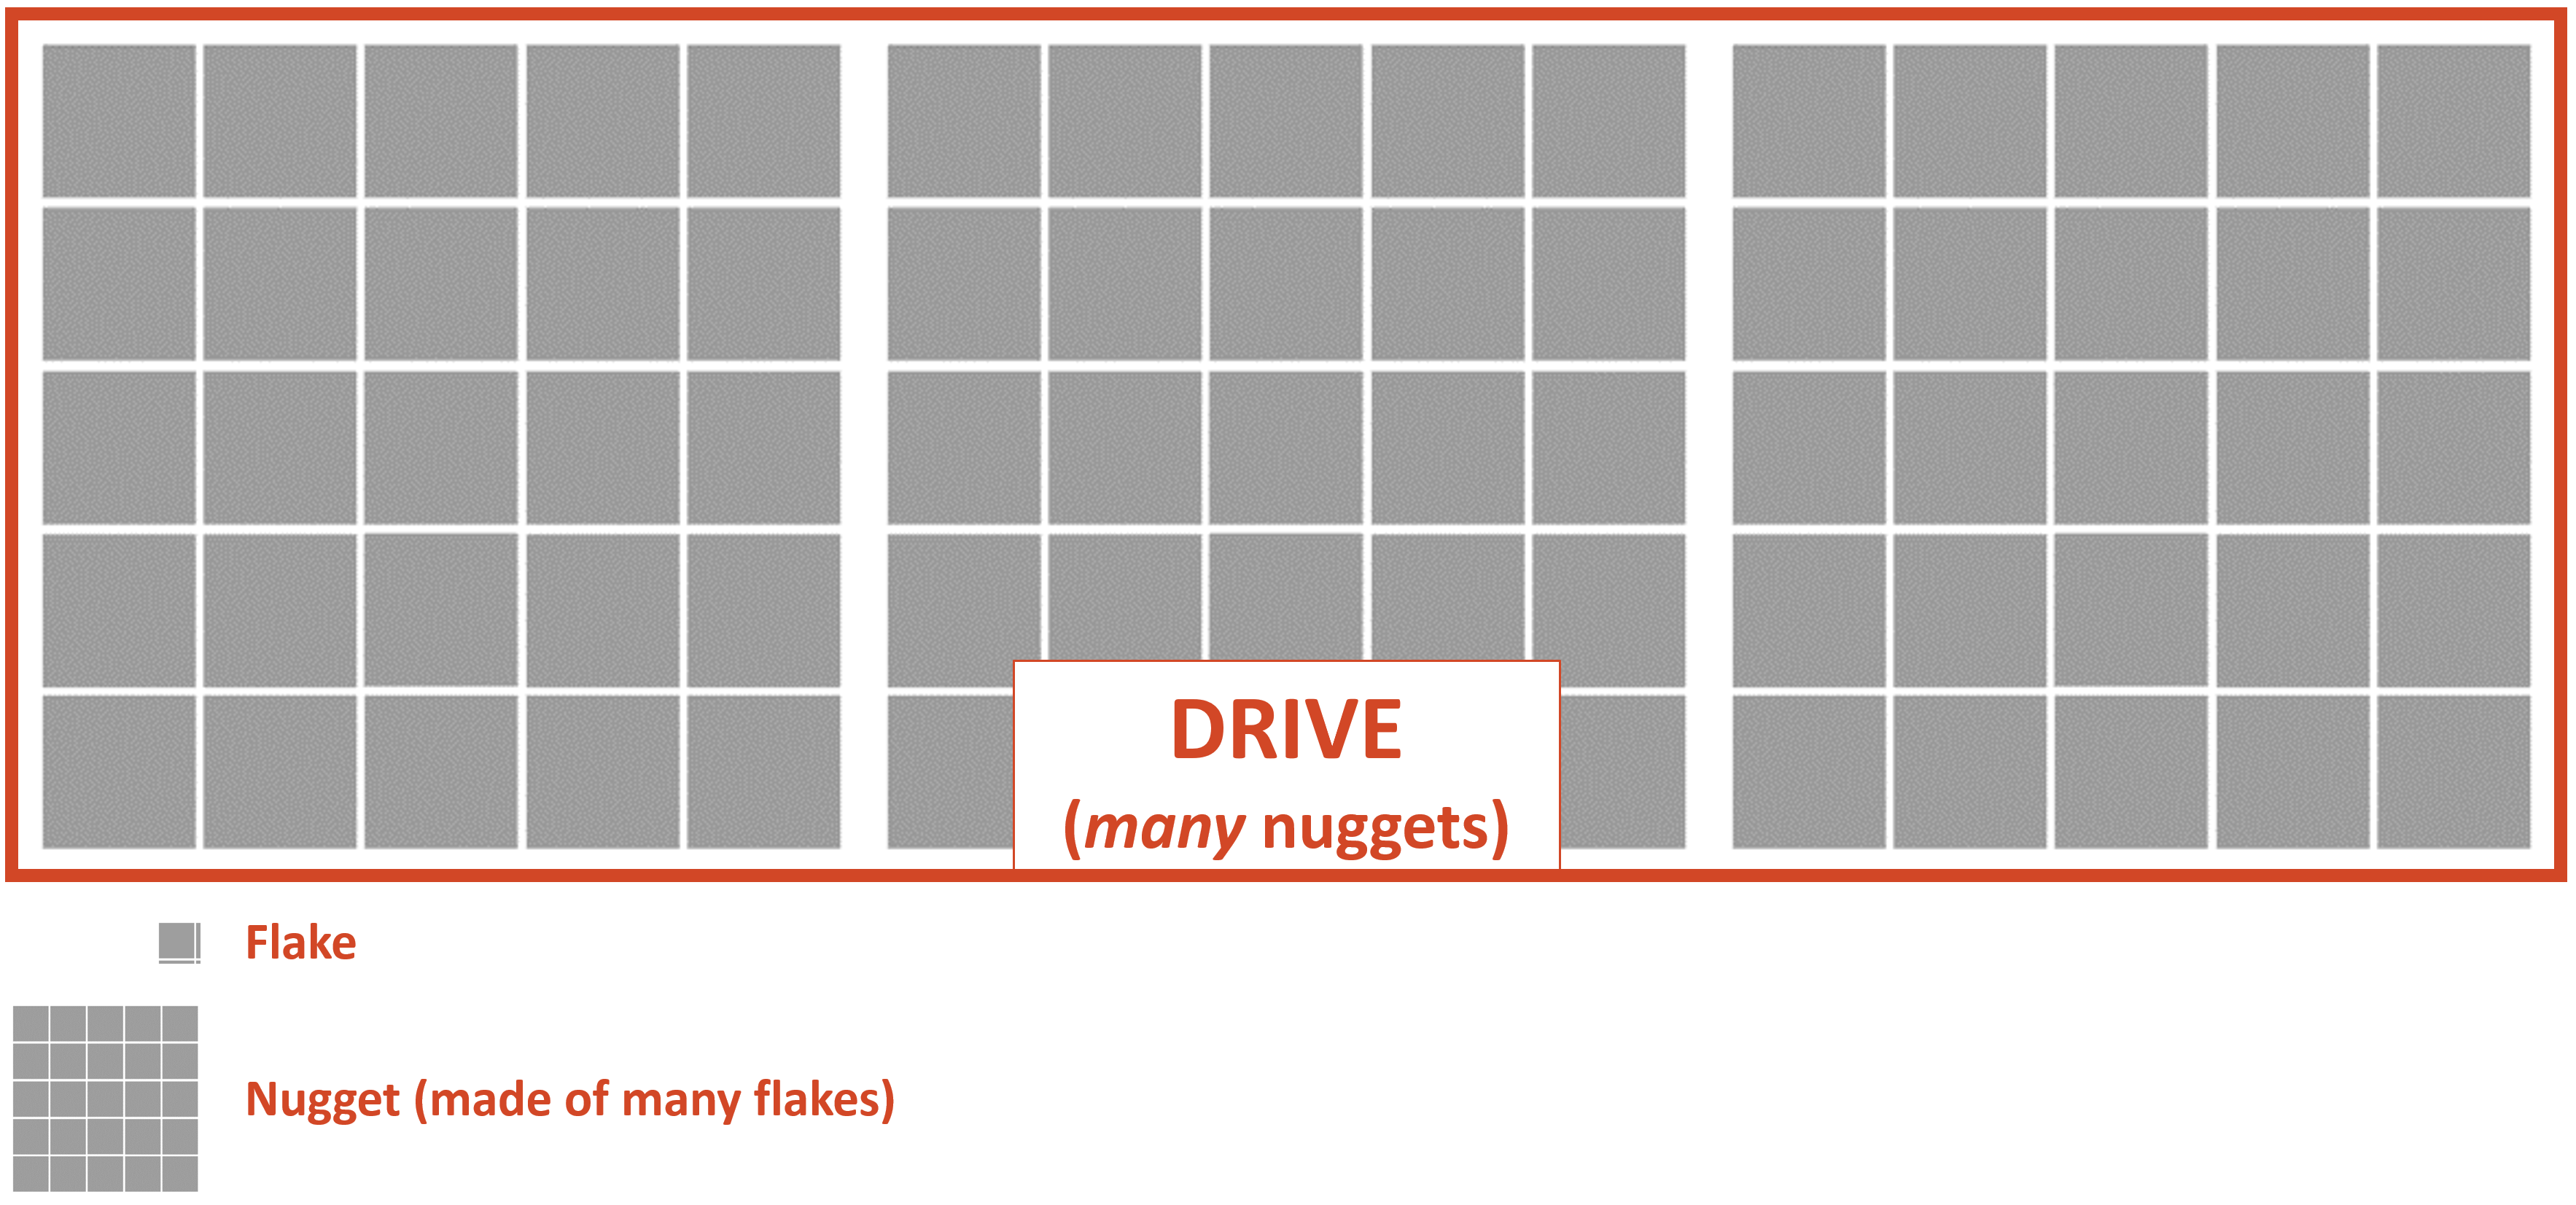
\includegraphics[width=\linewidth]{flknug.png}
   \caption{Anatomy of a StrongBox nugget.}\label{fig:flknug}
\end{figure}

StrongBox divides the underlying drive into a series same-size logical blocks
called \emph{nuggets}, illustrated in \figref{flknug}. A nugget consists of one
or more physical drive blocks/sectors, depending on its configured size. Each
nugget is subdivided into a constant number of blocks called \emph{flakes}.

This flake-nugget structure is used by StrongBox to 1) track, detect, and handle
overwrites and 2) limit the maximum length of any plaintexts provided to
ciphers, thus capping the per-cycle overhead incurred during expensive re-keying
operations when overwrites do occur.

\subsection{Key Insights}

\subsubsection{A Single Point In A Space Of Possible Cipher Configurations}

What if we used StrongBox with a cipher other than ChaCha20? Redesigning
StrongBox with a generic cipher API allows for ciphers other than ChaCha20 to be
used, yielding a space of cipher configuration points with various performance,
battery life, security, drive space, and other tradeoffs. It follows then that
the original StrongBox construction using ChaCha20 exists as one point in this
space of cipher configurations.

\begin{figure}[ht]
   \centering
   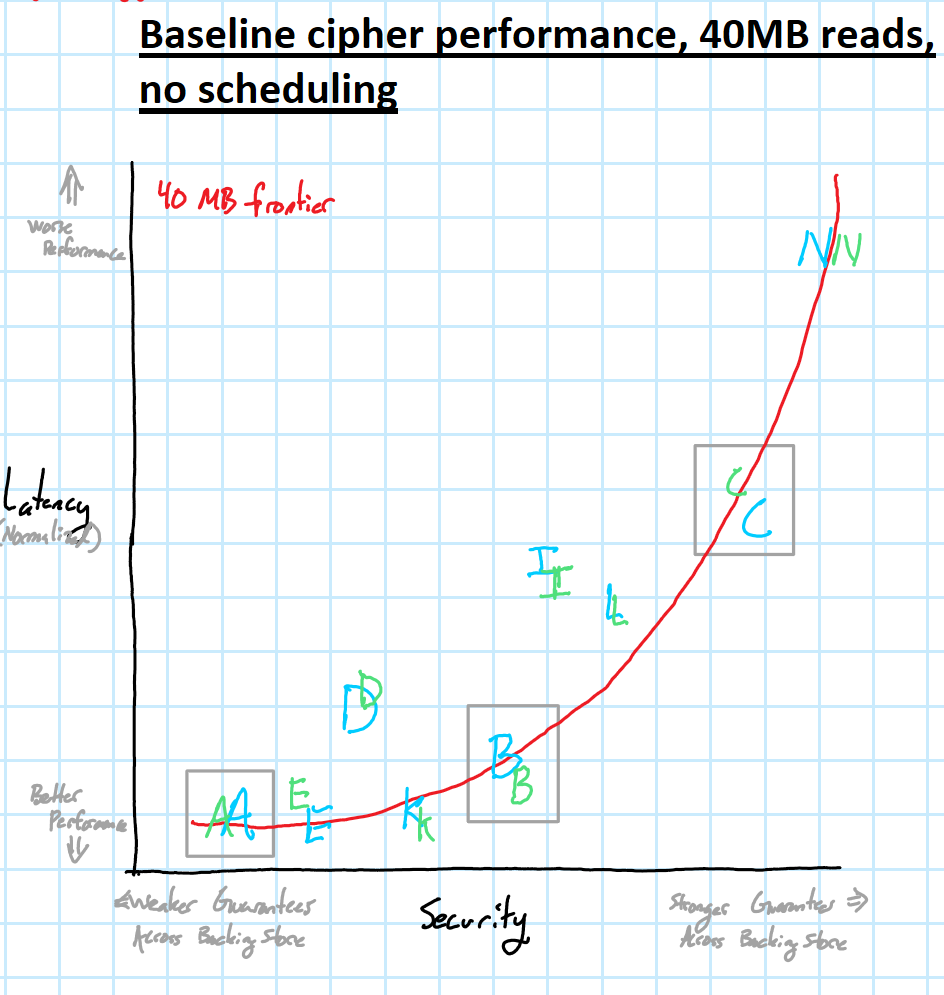
\includegraphics[width=\linewidth]{drawn/1.png}
   \caption{\TODO{Caption goes here}\TODO{No curve in this version!}}\label{fig:40mb-read}
\end{figure}

For instance, \figref{40mb-read} shows the security versus I/O latency tradeoff
between different stream ciphers (including ChaCha20) when completing a 40MB
read of encrypted storage. The experiment was performed on an ARM big.LITTLE
Exynos Octa processor, which is similar to the processors used in the Samsung
Galaxy line of phones and other devices. Of the ciphers we tested, those with
relatively stronger security guarantees resulted in higher latency for I/O
operations while ciphers with relatively weaker security guarantees resulted in
lower latency.

\subsubsection{Encryption And Re-Keying Of Nuggets Occur Entirely Independently}

With StrongBox, nuggets are considered as individual distinct logical blocks,
each with their own metadata and unique cryptographic key used to encrypt and
decrypt their contents with the single cipher chosen at initialization. This
layout naturally lends itself to encrypting different portions of the underlying
drive with different ciphers instead; we can select any cipher to encrypt or
decrypt any nugget at any point, rather than just a single cipher globally. This
allows the filesystem to support mixed cipher configurations that can be
encrypted, decrypted, swapped individually.

\subsubsection{Navigate The Configuration Space With ``Cipher Switching''}

Given a space of possible cipher configurations and a drive layout of
independent nuggets that lends itself to mixed cipher use, it is clear our
system does not have to sit at a static configuration point. Hence, we require a
mechanism to navigate the cipher configuration space, trading off concerns such
that the system is always at the most optimal configuration in context. By
abstracting the rekeying process out into a re-ciphering or \emph{cipher
switching} process, whereby the key and the cipher used to encrypt/decrypt the
nugget can both be switched at runtime, we can trade off between different
ciphers and their characteristics dynamically. Comparatively, prior work can
only accomplish a static tradeoff at compile time or at filesystem
initialization.
\\
\\
Leveraging these insights, we present SwitchBox. \TODO{A few short explanatory
sentences that lead to: Our goal is to dynamically trade security for
performance or energy.}

\subsection{Motivating Example: Reacting to OS ``Power Saver'' Mode}

\TODO{Talk about the energy-budget case study here as motivation.}

\subsection{Challenges}

\textbf{Comparing ciphers with disparate security guarantees.} To ensure that
these tradeoffs are made optimally, it is desirable to quantify the security of
various ciphers. This is challenging since different schemes are designed to
mitigate entirely disparate and unrelated threats. To address this, we propose a
method for quantitative cipher comparison in the FDE context, and then present
some empirical results showing the wide range of security and energy tradeoffs
that are available with state-of-the-art ciphers.
\\
\\
\textbf{Maintaining I/O performance with a mixed-cipher drive layout.} SwitchBox
requires a generic cipher API and novel IPC mechanism that can switch the
ciphers of individual nuggets while maintaining low overhead and acceptable
performance. This mechanism provides the ``how'' to switch a nugget's cipher,
but does not provide the ``when'' or ``where'' to do so; to address this, we
implement and demonstrate a series of cipher switching \textit{strategies} that
facilitate navigating our space of possible configurations. These strategies
allow SwitchBox to settle on points between the static configurations in
\figref{40mb-read}.
